
\chapter{METODOLOGI PENELITIAN}
\label{cha:3-MetodologiPenelitian}

\section{Gambaran Umum} \label{sec:3-GambaranUmum}

Penelitian ini membahas pemanfaatan data gambar sebagai acuan dalam melakukan pelatihan dan
implementasi model \textit{deep neural network} untuk mencari dan memetakan koordinat tiga dimensi
pose tubuh manusia dalam sebuah rangkaian gambar secara lokal. Pengerjaan aplikasi mengutamakan dua
langkah penting yang meliputi pengolahan data dan pembuatan model. Aplikasi yang dibuat dapat menampilkan
plot grafik tiga dimensi menyerupai struktur anatomi tubuh manusia sesuai dengan pose hasil
estimasi dari gambar masukkan. Hasil pelatihan model ditampilkan dalam grafik dua dimensi untuk
analisis lebih lanjut.

\textit{Dataset} yang digunakan dalam penelitian ini terbagi menjadi dua jenis yang meliputi
\textit{dataset} pembuatan model dan \textit{dataset} inferensi aplikasi.
\textit{Dataset} pembuatan model dikategorikan menjadi data pelatihan model dan data validasi model.
\textit{Dataset} pembuatan model berisi gambar dan target posisi titik kunci anatomi dalam jumlah besar.
Data pelatihan model adalah data yang digunakan dalam proses pelatihan sebagai sampel bagi \textit{deep neural network}.
Data validasi model adalah data yang digunakan untuk menguji kebenaran fungsionalitas pemetaan yang
dipelajari saat pelatihan model. \textit{Dataset} inferensi aplikasi adalah data uji coba berbentuk
video tanpa target titik kunci yang digunakan untuk estimasi pose tubuh manusia secara sekuensial.

Pelatihan model \textit{deep neural network} diimplementasikan menggunakan \textit{framework} PyTorch.
Kedua \textit{dataset} yang digunakan diolah terlebih dahulu sehingga memenuhi syarat PyTorch dalam melakukan
\textit{deep learning}.
Setiap model kemudian digunakan terhadap \textit{dataset} inferensi
aplikasi. Proses dan hasil estimasi diurai lebih lanjut dalam bentuk grafik visual.

\section{Kerangka Penelitian} \label{sec:3-KerangkaPenelitian}

Kerangka penelitian yang jelas dibutuhkan untuk memudahkan proses penelitian sehingga dapat
mempersingkat waktu pengerjaan. Proses penelitian dibagi menjadi tiga tahapan besar yang meliputi
tahap praproduksi, tahap produksi, dan tahap uji coba. Setiap tahapan tersebut dikerjakan secara
terurut dan sistematis. Alur setiap tahap diilustrasikan pada gambar~\ref{fig:kerangkapenelitian}.

\begin{figure}[htbp]
    \begin{center}
        \fbox{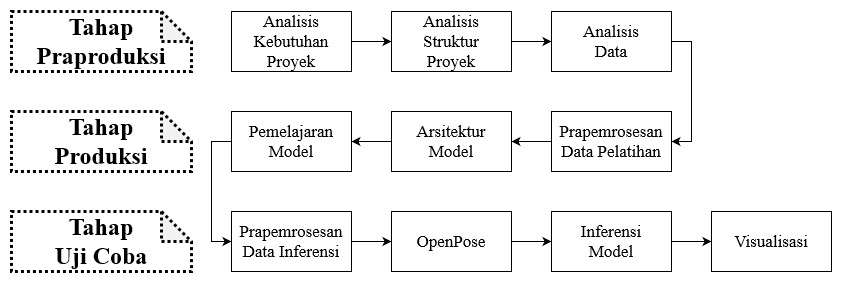
\includegraphics[width=11.9cm]{bab3/gambar/kerangka_penelitian.jpg}}
    \end{center}
    \vspace{-20pt}
    \captionsetup{labelfont=bf, textfont=bf}
    \caption{Kerangka Penelitian}
    \vspace{-10pt}
    \captionsetup{labelfont=md, textfont=md}
    % \caption*{Sumber: sumber}
    % \caption*{Sumber: Zhang (2019)}
    \label{fig:kerangkapenelitian}
\end{figure}

\section{Tahap Praproduksi} \label{sec:3-TahapPraproduksi}

\subsection{Analisis Kebutuhan Proyek}
Hardware dan software

\subsection{Analisis Struktur Proyek}
Struktur Folder

\subsection{Analisis Data}
Data Latihan
Data Inferensi

\section{Tahap Produksi} \label{sec:3-TahapProduksi}

\subsection{Prapemrosesan Data Pelatihan}
Kelas DataLoader

\subsection{Arsitektur Model}
DNN

\subsection{Pelatihan Model}


\section{Tahap Uji Coba} \label{sec:3-TahapUjiCoba}

\subsection{Prapemrosesan Data Inferensi}

\subsection{OpenPose}

\subsection{Inferensi Model}

\subsection{Visualisasi}

\begin{table}[htbp]
    \captionsetup{labelfont=bf, textfont=bf}
    \caption{Sebuah tabel}
    \vspace{-20pt}
    \begin{center}
        \begin{tabular}{| l c r |}
            \hline
            1 & 2 & 3 \\
            4 & 5 & 6 \\
            7 & 8 & 9 \\
            \hline
        \end{tabular}
    \end{center}
    \vspace{-10pt}
    \captionsetup{labelfont=md, textfont=md}
    % \caption*{Sumber: Bego Lu}
\end{table}